\documentclass[sigconf,nonacm]{acmart}

\usepackage{booktabs}
\usepackage{array}
\usepackage{pgfgantt}
\usetikzlibrary{arrows.meta}

\definecolor{coral}{HTML}{E2614A}
\definecolor{teamgray}{HTML}{8A8FA6}
\newcommand{\HRtwo}{\mathrm{HR}_2}

\begin{document}

\title{Generate-then-Select: Recovering Authorship Facts That LLMs Recognize but Fail to Recall}
\subtitle{CS 7980 Research Capstone --- Project Proposal (Generate-then-Select Track)}

\author{Minyan Xu}
\affiliation{%
  \institution{Northeastern University}
  \country{USA}}
% Other tracks of the same team project: Hana Feng (activation steering), Zhiqi Zhang (J-Lens).

\maketitle

%% ===================================================================
\section{Introduction}

Large language models (LLMs) often state wrong facts with confidence, and these errors concentrate on facts that are rare in their training data~\cite{kandpal2023longtail,mallen2023popqa,sun2024headtotail}. Zhong et al.~\cite{zhong2026dreaming} study this through academic authorship attribution: given a paper's title and publication year, the model must name its authors. Hallucination falls as a paper's citation count grows, but remains near-total in the long tail. Our team re-ran their open-question baseline with Qwen3-32B~\cite{qwen3} on the same 9,108-paper benchmark: only 1.41\% of papers receive a fully correct author list, matching the original run (1.45\%).

Yet the model often \emph{picks} authors it cannot \emph{name}. In our first-version recognition test, Qwen3-32B chose the true author list out of four options, in both of two shuffled orders, for 69\% of papers. Calderon et al.~\cite{calderon2026emptyshelves} report the same pattern at scale: frontier models encode 95--98\% of the facts they test but still fail to recall many of them. This points to a recall bottleneck rather than missing knowledge. There is a caveat, however: when we hid the title and kept the same four options, the model still picked the true list for 36\% of papers (chance $\approx$ 6\%). Multiple choice can thus be partly solved from cues in the options, so how much knowledge is truly latent is still an open measurement question.

\paragraph{Scope and relation to the team project.}
Our team asks whether such latent knowledge can be brought out at answer time without retraining. The project has one shared measurement and three method families (Figure~\ref{fig:logic}). The shared recognition test labels each paper as known and said, known but not said, or not known (team RQ1). Three method families then try to elicit what is known: activation steering (CAA, ITI, BiPO), which writes to internal states; J-Lens, which reads internal states and derives directions from them; and generate-then-select, which uses outputs only (team RQ2). All three are compared on the same held-out papers, by citation level (team RQ3). This proposal covers the generate-then-select track.

The phrase ``multiple choice'' names two different things in this project, and keeping them apart is what keeps the logic consistent. As a \emph{measurement}, multiple choice is the recognition test: the true answer is placed among distractors, and the result labels papers and sets the ceiling for every method. This part is shared and upstream of all three tracks; my contribution to it is a harder, better-controlled version (Stage~A). As a \emph{method}, multiple choice is the selection step of generate-then-select: the options are the model's own sampled answers, which may not contain the truth. This part is one of the three parallel elicitation approaches, not preparation for the others. It needs no labels to run and no access to model internals, which also makes it the baseline that the white-box approaches must beat at equal compute. Its failure analysis (Stage~B) feeds back into the shared labels by showing which failures can be fixed at the output level and which require intervening on internal states.

\begin{figure}[t]
\centering
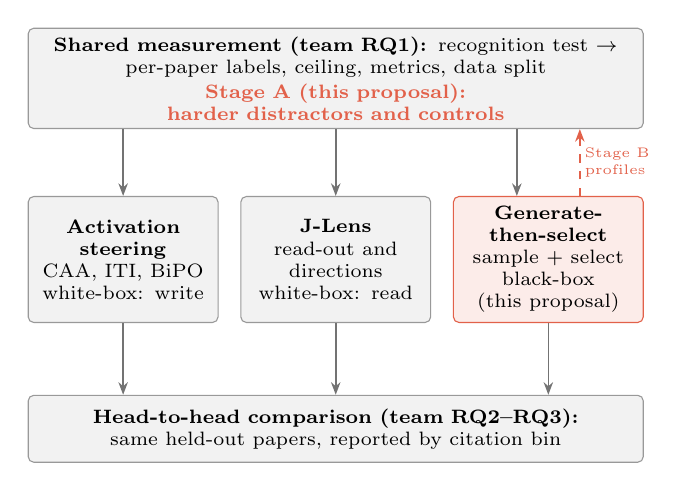
\begin{tikzpicture}[
  box/.style={draw=black!40, rounded corners=2pt, align=center, font=\scriptsize, inner sep=3pt},
  shared/.style={box, fill=black!5, text width=7.6cm, minimum height=0.85cm},
  method/.style={box, fill=black!5, text width=2.2cm, minimum height=1.6cm},
  mine/.style={method, fill=coral!12, draw=coral},
  arr/.style={-{Stealth[length=1.6mm]}, black!55, semithick}]
\node[shared] (S) at (0,0) {\textbf{Shared measurement (team RQ1):} recognition test $\rightarrow$\\per-paper labels, ceiling, metrics, data split\\[1pt]\textcolor{coral}{\textbf{Stage A (this proposal): harder distractors and controls}}};
\node[method] (St) at (-2.7,-2.3) {\textbf{Activation}\\\textbf{steering}\\CAA, ITI, BiPO\\white-box: write};
\node[method] (J)  at (0,-2.3)    {\textbf{J-Lens}\\read-out and\\directions\\white-box: read};
\node[mine]   (G)  at (2.7,-2.3)  {\textbf{Generate-}\\\textbf{then-select}\\sample + select\\black-box\\(this proposal)};
\node[shared] (C) at (0,-4.45) {\textbf{Head-to-head comparison (team RQ2--RQ3):}\\same held-out papers, reported by citation bin};
\draw[arr] (St.north |- S.south) -- (St.north);
\draw[arr] (J.north |- S.south) -- (J.north);
\draw[arr] ([xshift=-0.4cm]G.north |- S.south) -- ([xshift=-0.4cm]G.north);
\draw[arr, dashed, coral] ([xshift=0.4cm]G.north) -- ([xshift=0.4cm]G.north |- S.south)
  node[midway, right, font=\tiny, text=coral, inner sep=1.5pt, align=left] {Stage B\\profiles};
\draw[arr] (St.south) -- (St.south |- C.north);
\draw[arr] (J.south) -- (J.south |- C.north);
\draw[arr] (G.south) -- (G.south |- C.north);
\end{tikzpicture}
\caption{How this track fits the team project. The recognition test (top) is shared measurement that labels papers and sets the ceiling for every method; Stage~A hardens it. The three method families run in parallel, and generate-then-select is the only black-box one. Stage~B's failure profiles flow back into the shared labels (dashed). All methods are compared on the same held-out papers (bottom).}
\label{fig:logic}
\end{figure}

\paragraph{Framework.}
Memory research distinguishes knowledge that is stored from knowledge that can be retrieved~\cite{tulving1966availability}, and describes recall as two steps: generating candidates, then recognizing the right one~\cite{kintsch1970models,anderson1972recognition}. Accordingly, a wrong greedy answer has two possible causes. In a \emph{generation failure}, the correct author is never produced. In a \emph{selection failure}, it is produced in some samples but not chosen. Generate-then-select addresses selection failures with an explicit selection step, and generation failures with more diverse generation.

\paragraph{Research questions.}
\begin{itemize}
\item \textbf{RQ1 (Measurement).} Once shortcut cues are controlled, how large is the gap between recognizing and recalling a paper's authors, and how does it change with citation count? (Contributes to team RQ1.)
\item \textbf{RQ2 (Decomposition).} Among recall failures, what share are generation failures and what share are selection failures, and how does this mix change with citation count?
\item \textbf{RQ3 (Elicitation).} Can generate-then-select recover authors that the model recognizes but does not recall, beating direct answering, self-consistency, and chain-of-thought at matched compute? How does it compare with the team's white-box methods on the same held-out papers? (Contributes to team RQ2--RQ3.)
\end{itemize}

\noindent The expected outcomes are a harder recognition test with per-paper labels shared by the team; a per-paper split of recall failures across 13 citation bins; and a black-box elicitation method with compute-matched evaluation, which also serves as the team's baseline.

%% ===================================================================
\section{Related Work}

\paragraph{Long-tail factual knowledge.}
LLMs answer questions about popular entities far better than about rare ones. QA accuracy tracks the number of relevant pretraining documents~\cite{kandpal2023longtail}; models struggle most with less popular entities, where retrieval helps most~\cite{mallen2023popqa}; and accuracy drops from head to torso to tail facts~\cite{sun2024headtotail}. Zhong et al.~\cite{zhong2026dreaming} use citation count as a proxy for how often an authorship fact appears in training data. They find a robust inverse relation between citations and hallucination, together with much higher multiple-choice recognition than open-ended recall.

\paragraph{Latent versus expressed knowledge.}
Calderon et al.~\cite{calderon2026emptyshelves} separate encoding from recall at the level of individual facts: rare facts are usually encoded but hard to recall, reverse questions are recognized but hard to answer, and thinking recovers part of the failures. Gekhman et al.~\cite{gekhman2025insideout} show that models know more internally than they express, and that some answers are almost never sampled even though the model would rank them first if they appeared. Orgad et al.~\cite{orgad2025llms} train verifiers on hidden states to choose among sampled answers. We study the same gap on a much longer tail and split it into generation and selection failures along a prevalence axis.

\paragraph{Sampling and selection.}
Self-consistency takes the most frequent answer among samples~\cite{wang2023selfconsistency}. Models can also judge their own samples through P(True), and judge better after seeing several samples~\cite{kadavath2022language}. We estimate coverage with the unbiased pass@$k$ estimator~\cite{chen2021codex}, correct likelihoods for surface-form frequency with PMI~\cite{holtzman2021surface}, and test scoring in the authors-to-title direction because the direction of a query affects what models can retrieve~\cite{berglund2024reversal}.

\paragraph{Pitfalls of multiple-choice evaluation.}
LLMs often answer multiple-choice questions from the options alone~\cite{balepur2024artifacts} and prefer certain option positions or letters~\cite{zheng2024mcq}. Our distractor ladder, controls, and order permutations target exactly these effects.

\paragraph{White-box elicitation.}
The other two tracks of our team intervene on internal states. Activation steering adds directions to activations at inference time, built from contrastive pairs~\cite{rimsky2024caa}, from selected attention heads~\cite{li2023iti}, or by optimization~\cite{cao2024bipo}; lens-based methods read out intermediate states. Generate-then-select needs only model outputs and serves as their black-box counterpart and baseline.

%% ===================================================================
\section{Methods}

The track has three stages. Stage~A hardens the shared recognition test (RQ1), Stage~B splits recall failures into generation and selection failures (RQ2), and Stage~C builds and evaluates generate-then-select methods (RQ3). The methods section describes approaches to investigate rather than a fixed solution.

\subsection{Data, Model, and Shared Setup}

We use the 9,108-paper benchmark of Zhong et al.~\cite{zhong2026dreaming}: up to 100 papers per field and citation bin, over 8 fields and 13 exponentially spaced citation bins, with titles, years, and Semantic Scholar author lists as ground truth. Our main model is Qwen3-32B~\cite{qwen3}, the open-weight model the whole team uses. It exposes token log-probabilities, which several scoring functions need, and it has both a thinking and a non-thinking mode, which provides a natural chain-of-thought baseline. Inference uses vLLM~\cite{kwon2023vllm}. If API access allows, we also replicate the original multiple-choice test on GPT-4o to connect with the 79\% chance-corrected accuracy that~\cite{zhong2026dreaming} report for rarely cited papers. The first author is the primary target, since a single entity keeps sampling and scoring clean; full author lists follow once the pipeline is stable.

We share the team's labels, metrics, and data split. The team splits the 3,341 ``known but not said'' papers from its first recognition test into build (50\%), tune (10\%), and test (40\%) parts. Generate-then-select has nothing to build, so it uses the tune part to choose hyperparameters (number of samples, temperature, thresholds) and reports on the same test part, which keeps the head-to-head comparison fair. Because these papers were themselves selected with a multiple-choice test, we also report results on all 9,108 papers, so that a selection-based method is not evaluated only on papers chosen for being easy to select.

\subsection{Stage A: A Harder Recognition Test (RQ1)}

The first recognition test used random same-field names as distractors, and the title-hidden control shows that they leak cues. Stage~A replaces them with a ladder of harder distractors (Table~\ref{tab:ladder}). Each level removes one more shortcut that would allow a correct pick without knowing the paper. For L1--L3, teams that share an author with the true team are excluded, and all options are normalized to one name format (``F.~Lastname'') so that formatting is not itself a cue.

\begin{table}[t]
\caption{Distractor ladder for the recognition test.}
\label{tab:ladder}
\small
\begin{tabular}{@{}>{\raggedright\arraybackslash}p{0.75cm}>{\raggedright\arraybackslash}p{3.45cm}>{\raggedright\arraybackslash}p{3.0cm}@{}}
\toprule
Level & Distractors & Shortcut removed \\
\midrule
L0 & Random same-field names (first-test design) & none (reference level) \\
L1 & Real team of another same-field paper, same number of authors & team coherence (same lab, same language background) \\
L2 & L1, with publication year within $\pm$2 & era and name-format cues \\
L3 & L2, from the most similar title, matched on team prominence & topic and famous-name cues \\
L4 & True team with one author swapped for a real collaborator & knowing the group but not the paper \\
L5 & The model's own wrong answers & hardest; matches the method setting \\
\bottomrule
\end{tabular}
\end{table}

Three controls should each stay near chance: \emph{title hidden} (options only, already run in the first test), \emph{title swap} (the same options paired with another paper's title from the same field and period), and \emph{catch trials} (the true answer removed and ``none of the above'' correct), which measure false recognition. Choices-only shortcuts~\cite{balepur2024artifacts} are tracked by these controls. To remove position bias~\cite{zheng2024mcq}, each item is asked in all four cyclic option orders and counted as recognized only if it is answered correctly in most of them.

Besides joint multiple choice, we ask a yes/no question for each candidate, which separates discrimination ($d'$) from a general tendency to answer ``yes''~\cite{green1966sdt}. We also score candidates by their likelihood, in coordination with the team's filter based on true-author probability. The main metric is pairwise AUC: the fraction of (correct, incorrect) candidate pairs in which the correct one scores higher~\cite{gekhman2025insideout}. It equals the expected accuracy of a two-alternative forced choice, does not depend on a threshold, and applies to all three formats. As a reliability check, a 2$\times$2 table of recalled versus recognized papers should contain almost no papers that are recalled but not recognized. Stage~A outputs recognition curves by citation bin for each ladder level and a per-paper label, ``recognized under hard distractors,'' which sharpens the team's filter.

\subsection{Stage B: Splitting Recall Failures (RQ2)}

For each paper, we take the greedy answer and $n$ samples at several temperatures ($n$ up to 100; $T \in \{0.7, 1.0, 1.3\}$). Coverage@$k$ is the probability that the correct first author appears in at least one of $k$ samples. From $n$ samples with $c$ correct ones, it is estimated without bias as~\cite{chen2021codex}
\[
\text{coverage@}k \;=\; 1 - \binom{n-c}{k} \Big/ \binom{n}{k}.
\]
The matching rule (last name plus first initial) lets common surnames match by luck as $k$ grows. We therefore compute a chance baseline by matching each paper's samples against the true authors of a different paper from the same field and period, and report coverage net of this baseline.

Each paper then falls into one of four profiles:
\begin{itemize}
\item \emph{Direct recall}: the greedy answer is correct.
\item \emph{Reachable}: the greedy answer is wrong, but the correct author appears among the samples, so selection can fix it.
\item \emph{Recognized but unreachable}: the correct author is never sampled but is recognized in Stage~A, so generation must improve.
\item \emph{Not recognized}: recognition fails even with hard distractors, so the fact is probably not stored.
\end{itemize}
The key result is the share of each profile by citation bin, for several values of $k$. It shows where recoverable knowledge lies, whether recovering it needs better selection or better generation, and where knowledge appears to be absent. The profiles are added to the shared labels. Reachable papers mark what output-level methods can fix. Recognized-but-unreachable papers mark where steering and J-Lens have room that sampling cannot reach. Not-recognized papers act as a negative control for all methods, since a method that ``recovers'' them is likely guessing.

\subsection{Stage C: Generate-then-Select (RQ3)}

\paragraph{Generation (raising coverage).}
We compare temperature and top-$p$ sweeps; prompt formats (question--answer, a database-style ``Title: \ldots{} Authors:'' entry, and reference-list style); exclusion prompting, which asks for an author not already listed; decomposed generation (the first author alone, or co-authors given one author); and first-letter cues. Giving the model the true first letter leaks information, so it serves only as a diagnostic. Enumerating letters, or the most likely first tokens of the surname, and then selecting leaks nothing and is a legitimate method. All strategies are compared at equal compute.

\paragraph{Selection (choosing from the pool).}
We compare five scoring functions:
\begin{itemize}
\item joint multiple choice over the unique candidates, with a ``none of the above'' option that allows abstention;
\item P(True) for each candidate~\cite{kadavath2022language};
\item PMI-corrected likelihood, $\log P(a \mid t) - \log P(a \mid \emptyset)$ for candidate author $a$ and title $t$, which removes the prior that common names are more probable~\cite{holtzman2021surface};
\item scoring in the authors-to-title direction, $\log P(t \mid a) - \log P(t \mid \emptyset)$, with the authors placed in a reference-list format, motivated by the reversal curse~\cite{berglund2024reversal} and by the finding that reverse questions are recognized but hard to recall~\cite{calderon2026emptyshelves};
\item majority vote (self-consistency~\cite{wang2023selfconsistency}) as the baseline.
\end{itemize}
For full author lists, names are pooled across samples, scored one by one, and kept if their score clears a threshold tuned on the tune split.

\subsection{Evaluation Metrics and Experiments}

\paragraph{Metrics.}
For recognition, we report chance-corrected accuracy and pairwise AUC by ladder level and citation bin. For the decomposition, we report net coverage@$k$ and the share of each profile. For elicitation, the main metric is first-author accuracy. For full lists, we count matched ($M$), made-up ($H$), and missed ($U$) names and report the hallucination rate $\HRtwo = (H+U)/(M+H+U)$ of~\cite{zhong2026dreaming}, together with the share of papers with all authors right. We also report selection accuracy given coverage, computed only on papers whose pool contains the answer, and selection efficiency, $(\mathrm{acc}_{\mathrm{select}} - \mathrm{acc}_{\mathrm{greedy}}) / (\mathrm{coverage} - \mathrm{acc}_{\mathrm{greedy}})$, which is the share of the reachable gap actually recovered.

\paragraph{Experiments.}
Baselines are greedy direct answering with the few-shot prompt of~\cite{zhong2026dreaming}, Qwen3's thinking mode as the chain-of-thought baseline, and self-consistency over $k$ samples. All comparisons are compute-matched: we plot accuracy against the number of generated tokens. We also plot accuracy against answer rate when the method may abstain, since avoiding confident fabrication is itself a goal. The key ablation is whether selection beats majority vote; if it does not, the recognition step adds nothing beyond answer frequency. For the team comparison, results are reported on the shared test split and by citation bin. Methods are compared on the same papers with paired bootstrap or McNemar tests. Regressions use mixed-effects logistic models with paper and field random effects, controlling for author prominence, surname commonness, publication year, title specificity, and number of authors.

\paragraph{Resources.}
Qwen3-32B in bf16 needs about 65\,GB of GPU memory, so it fits on one 80\,GB GPU or on two smaller GPUs with tensor parallelism. With the first author as target, 50 samples for each of the 9,108 papers amount to about 0.46 million short generations. With parallel sampling in vLLM, each configuration takes a few GPU-hours, and the full plan needs on the order of tens of GPU-hours. The optional GPT-4o replication needs about 36{,}000 short API calls (9,108 papers $\times$ 4 option orders).

\paragraph{Risks and decision points.}
If recognition of rarely cited papers falls to chance under hard distractors, recoverable knowledge is concentrated in the middle citation bins, and the methods will focus there. If it stays high while all controls are at chance, the deep tail holds latent knowledge, and cue-based generation becomes central. If recognized-but-unreachable papers dominate, sampling has reached its ceiling, and these papers become the main target for the steering and J-Lens tracks. If selection is no better than majority vote, the track will shift its emphasis to generation and measurement.

%% ===================================================================
\section{Execution Timeline}

Figure~\ref{fig:gantt} shows the schedule, which is aligned with the team timeline and the course deliverables. Rows under ``Whole team'' are shared work; rows under ``Minyan Xu'' are my responsibilities. The pilot (weeks of 10/5 to 10/19) samples many answers to check that the true authors appear, and sets up the pipeline for name normalization, matching, and scoring. Stage~A is due at Update~1 (10/26) and Stage~B at Update~2 (11/9). Stage~C delivers first results to the team's full comparison at Update~3 (11/16) and is complete by the draft paper (11/30).

\begin{figure*}[t]
\centering
\resizebox{\textwidth}{!}{%
\begin{ganttchart}[
  hgrid, vgrid,
  x unit=1.2cm, y unit title=0.55cm, y unit chart=0.55cm,
  title/.append style={fill=black!6, draw=black!25},
  title label font=\footnotesize\bfseries,
  bar/.append style={fill=teamgray, draw=none},
  bar height=0.5, bar top shift=0.25,
  bar label font=\footnotesize,
  group/.append style={fill=black!70, draw=none},
  group height=0.22, group top shift=0.39,
  group label font=\footnotesize\bfseries,
]{1}{11}
\gantttitle{10/5}{1}\gantttitle{10/12}{1}\gantttitle{10/19}{1}\gantttitle{10/26}{1}\gantttitle{11/2}{1}\gantttitle{11/9}{1}\gantttitle{11/16}{1}\gantttitle{11/23}{1}\gantttitle{11/30}{1}\gantttitle{12/7}{1}\gantttitle{12/14}{1} \\
\gantttitle[title label font=\scriptsize\itshape]{Proposal}{1}%
\gantttitle{}{1}%
\gantttitle[title label font=\scriptsize\itshape]{Intro/RW}{1}%
\gantttitle[title label font=\scriptsize\itshape]{Update 1}{1}%
\gantttitle{}{1}%
\gantttitle[title label font=\scriptsize\itshape]{Update 2}{1}%
\gantttitle[title label font=\scriptsize\itshape]{Update 3}{1}%
\gantttitle{}{1}%
\gantttitle[title label font=\scriptsize\itshape]{Draft}{1}%
\gantttitle{}{1}%
\gantttitle[title label font=\scriptsize\itshape]{Final talk}{1} \\
\ganttgroup{Whole team (shared)}{1}{11} \\
\ganttbar{Recognition test + baseline, first version (done)}{1}{1} \\
\ganttbar{Shared paper labels, metrics, train/test split}{1}{2} \\
\ganttbar{Report: introduction, related work, methods, results}{2}{9} \\
\ganttbar{Final report, poster, video, presentation}{9}{11} \\
\ganttgroup{Minyan Xu (generate-then-select)}{1}{9} \\
\ganttbar[bar/.append style={fill=coral}]{Pilot: sample many answers, check coverage}{1}{3} \\
\ganttbar[bar/.append style={fill=coral}]{Stage A: harder recognition test with controls}{2}{4} \\
\ganttbar[bar/.append style={fill=coral}]{Stage B: split failures (never generated vs.\ not chosen)}{4}{6} \\
\ganttbar[bar/.append style={fill=coral}]{Stage C: selection methods vs.\ baselines at equal cost}{6}{9} \\
\ganttbar[bar/.append style={fill=coral}]{Results into the team's head-to-head comparison}{7}{9}
\end{ganttchart}%
}
\caption{Execution timeline (week of each Monday class). The second header row marks course deliverables. Gray bars are shared team work; coral bars are the responsibility of Minyan Xu.}
\label{fig:gantt}
\end{figure*}

%% ===================================================================
\bibliographystyle{ACM-Reference-Format}
\bibliography{references}

\end{document}
